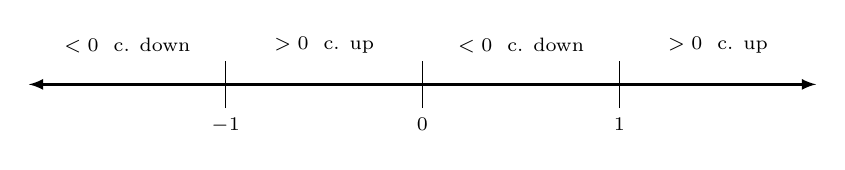
\begin{tikzpicture}[>=latex]

\draw [<->, thick] (-5,0) -- (5,0);
\foreach \x / \y  in %
					{%
					-2.5/{$-1$},%
					0/{$0$},%
					2.5/{$1$}%
					}
		{\draw (\x,-.3) node[below] {\scriptsize \parbox{40pt}{\centering \y}} -- (\x,.3);}
		
\draw (-3.75,.5) node {\scriptsize \parbox{50pt}{\centering $\fpp<0$ \ c. down }};
\draw (-1.25,.5) node {\scriptsize \parbox{50pt}{\centering $\fpp>0$ \ c. up }};
\draw (1.25,.5) node {\scriptsize \parbox{50pt}{\centering $\fpp<0$ \ c. down }};
\draw (3.75,.5) node {\scriptsize \parbox{50pt}{\centering $\fpp>0$ \ c. up}};


\end{tikzpicture}



